\documentclass[11pt,a4paper]{article}

\usepackage[margin=2.2cm]{geometry}
\usepackage[T1]{fontenc}
\usepackage[utf8]{inputenc}
\usepackage{lmodern}
\usepackage{microtype}
\usepackage{amsmath,amssymb,mathtools}
\usepackage{booktabs,array,tabularx}
\usepackage{xcolor}
\usepackage{tcolorbox}
\tcbuselibrary{skins,breakable}
\usepackage{tikz}
\usetikzlibrary{arrows.meta,positioning,shapes.geometric}
\usepackage{fancyhdr}
\usepackage{hyperref}
\usepackage{enumitem}

% Color palette (clean academic navy & slate)
\definecolor{navy}{HTML}{1B365D}
\definecolor{slate}{HTML}{2C5282}
\definecolor{tint}{HTML}{F4F7FA}
\definecolor{amber}{HTML}{8A5A00}
\definecolor{ambertint}{HTML}{FFFBEB}
\definecolor{greenink}{HTML}{1E5631}
\definecolor{greentint}{HTML}{F1F8F4}
\definecolor{bordergray}{HTML}{CBD5E1}

\hypersetup{
  colorlinks=true,
  linkcolor=slate,
  urlcolor=slate,
  pdftitle={Class Notes: Generalized Symbolic and Numerical Equation Formulation},
  pdfauthor={eqform Lecture Notes}
}

% Header / Footer
\pagestyle{fancy}
\fancyhf{}
\fancyhead[L]{\small\color{slate}\textsc{Class Notes: Generalized Equation Formulation (\texttt{eqform})}}
\fancyhead[R]{\small\color{slate}From Qualitative Dependencies to Calibrated Laws}
\fancyfoot[C]{\small\thepage}
\renewcommand{\headrulewidth}{0.4pt}

% Styled Callout Boxes
\newtcolorbox{setupbox}[1]{
  breakable,
  enhanced,
  colback=tint,
  colframe=navy,
  boxrule=0.8pt,
  arc=3pt,
  left=8pt,right=8pt,top=6pt,bottom=6pt,
  fonttitle=\bfseries\color{white},
  title={#1}
}

\newtcolorbox{insightbox}[1]{
  breakable,
  enhanced,
  colback=ambertint,
  colframe=amber,
  boxrule=0.8pt,
  arc=3pt,
  left=8pt,right=8pt,top=6pt,bottom=6pt,
  fonttitle=\bfseries\color{white},
  title={#1}
}

\newtcolorbox{resultbox}[1]{
  breakable,
  enhanced,
  colback=greentint,
  colframe=greenink,
  boxrule=0.8pt,
  arc=3pt,
  left=8pt,right=8pt,top=6pt,bottom=6pt,
  fonttitle=\bfseries\color{white},
  title={#1}
}

\tikzset{
  varnode/.style={circle, draw=navy, fill=tint, thick, minimum size=8.5mm, font=\small\bfseries},
  paramnode/.style={rectangle, rounded corners=3pt, draw=amber, fill=ambertint, thick, minimum height=7mm, inner sep=4pt, font=\small},
  targetnode/.style={circle, draw=greenink, fill=greentint, very thick, minimum size=9mm, font=\small\bfseries},
  dep/.style={-{Stealth[length=2.5mm]}, thick, color=navy},
  paramdep/.style={-{Stealth[length=2.2mm]}, dashed, thick, color=amber}
}

\newcommand{\dd}{\mathrm{d}}
\newcommand{\pd}[2]{\frac{\partial #1}{\partial #2}}
\newcommand{\td}[2]{\frac{\dd #1}{\dd #2}}
\newcommand{\dimbr}[1]{\left[#1\right]}

\title{
  {\color{navy}\rule{\textwidth}{1.8pt}}\\[0.6em]
  {\LARGE\bfseries\color{navy} Lecture Notes: Generalized Equation Formulation}\\[0.3em]
  {\large\color{slate} Symbolic Derivation \& Numerical Calibration from Qualitative Dependencies}\\[0.4em]
  {\color{navy}\rule{\textwidth}{0.8pt}}
}
\author{Companion Notes to \texttt{ch1.tex} and the \texttt{eqform} Solver (\texttt{python3 -m eqform.examples.ch1\_reproductions})}
\date{\today}

\begin{document}
\maketitle

\begin{abstract}
\noindent In many research and engineering problems, we know \emph{which} factors influence a target quantity long before we know the exact mathematical law connecting them. Extending the ``Alien Principle'' introduced in \texttt{ch1.tex}, these class notes present a generalized, domain-agnostic framework—implemented in the \texttt{eqform} symbolic and numerical solver—that converts qualitative dependency graphs (e.g., $g = \Phi(a,b,c)$ and $b = \psi(f)$) and optional unit dimensions into closed-form differential equations, integrated candidate laws, Buckingham-$\Pi$ dimensionless groups, and empirically calibrated models. We walk step by step through six worked examples executed directly by \texttt{eqform}.
\end{abstract}

\tableofcontents
\vspace{0.8em}
\hrule
\vspace{1em}

% ============================================================================
\section{Core Methodology: The 5-Step Generalized Recipe}
% ============================================================================

Suppose a researcher has \emph{no known equation}, only qualitative domain knowledge:
\begin{quote}
\emph{``Target factor $g$ depends on factors $a, b, c$, and factor $b$ in turn depends on $f$.''}
\end{quote}
To express $g$ explicitly as a function of $f$, \texttt{eqform} generalizes \texttt{ch1.tex} (which differentiated exclusively with respect to time $t$ and matched units by inspection) into a five-stage formal pipeline:

\begin{enumerate}[leftmargin=1.5em,itemsep=4pt]
  \item \textbf{Dependency DAG Construction}: Represent variables and governing constants as a Directed Acyclic Graph (DAG). An arrow $u \to v$ means $v$ depends on $u$. Cycles are rejected so bottom-up composition is well-defined.
  \item \textbf{Total Differential \& Active Path Pruning}: Expand the exact multivariate chain rule with respect to the query variable $f$:
  \begin{equation}
    \td{g}{f} = \sum_{x_i \in \text{parents}(g)} \pd{g}{x_i}\td{x_i}{f}.
  \end{equation}
  Any parent $x_i$ with no directed path from $f$ has $\td{x_i}{f} = 0$ and drops out of the active sum—\emph{crucially}, however, $x_i$ remains inside the partial derivative coefficients $\beta_i = \pd{g}{x_i}$ and integration baseline $g_0$.
  \item \textbf{Algebraic Dimensional Closure \& Buckingham-$\Pi$ Nullspace}: If dimensions are known (SI units \emph{or} custom domain units such as \texttt{USD}, \texttt{Users}, \texttt{Month}), each partial derivative $\beta_i = \pd{g}{x_i}$ must satisfy dimensional homogeneity:
  \begin{equation}
    \dimbr{\beta_i} = \frac{\dimbr{g}}{\dimbr{x_i}} \implies D\,\boldsymbol{\alpha} = \mathbf{d}_g - \mathbf{d}_{x_i},
  \end{equation}
  where columns of $D \in \mathbb{Q}^{k\times m}$ are the dimension vectors of the node's scope variables.
  \begin{itemize}[leftmargin=1.4em]
    \item \emph{Nullity $= 0$}: Unique monomial closure $\beta_i = \kappa_i \prod_j x_j^{\alpha_j}$.
    \item \emph{Nullity $= r > 0$}: The kernel $\ker(D)$ automatically yields $r$ dimensionless Buckingham-$\Pi$ groups $\{\Pi_1,\dots,\Pi_r\}$, generating $\Pi$-modulated candidate families (power-law $\prod_m \Pi_m^{\nu_m}$ and affine $1 + \sum_m \lambda_m \Pi_m$).
    \item \emph{No dimensions given}: Falls back cleanly to structural closures—first-order affine regression (Taylor ansatz) and constant-elasticity power-law scaling.
  \end{itemize}
  \item \textbf{Clairaut Exactness Coupling \& Integration}: For a conservative state function $u(x_1,\dots,x_m)$, mixed partial derivatives must commute:
  \begin{equation}
    \pd{\beta_i}{x_j} = \pd{\beta_j}{x_i} \qquad \forall\, i < j.
  \end{equation}
  Solving this linear system couples separate unknown constants $\kappa_i$ automatically (reducing free parameters!), after which Poincar\'e line integration reconstructs $u(x_1,\dots,x_m)$ and bottom-up substitution yields $g(f)$.
  \item \textbf{Numerical Calibration \& BIC Selection}: Unknown dimensionless constants ($\kappa_i$), offsets ($g_0$), and $\Pi$-group exponents ($\nu_m$) are estimated from data via exact SVD Ordinary Least Squares (when parameter-linear) or analytic-Jacobian Trust-Region Nonlinear Least Squares, and competing candidates are ranked by Bayesian Information Criterion (BIC).
\end{enumerate}

% ============================================================================
\section{Case 1A: Nested Dependency Graph Without Dimensions}
% ============================================================================

\begin{setupbox}{Problem Statement — Pure Qualitative Inference}
\textbf{Given}: $g = \Phi(a, b, c)$ and $b = \psi(f)$. No prior equations and \textbf{no physical dimensions} are known.\\
\textbf{Goal}: Express how $g$ varies with $f$, and construct candidate structural equations $g(f; a, c)$ that eliminate the intermediate variable $b$.
\end{setupbox}

\begin{center}
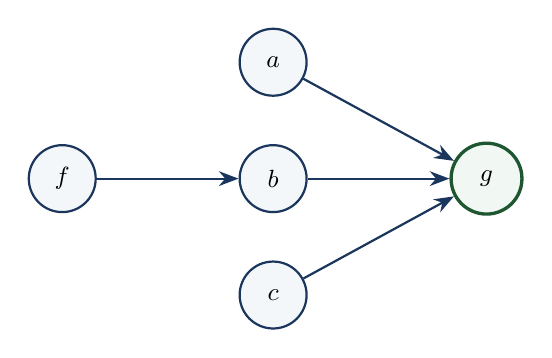
\begin{tikzpicture}[node distance=1.4cm and 1.8cm]
  \node[varnode] (f) {$f$};
  \node[varnode, right=of f] (b) {$b$};
  \node[varnode, above=0.6cm of b] (a) {$a$};
  \node[varnode, below=0.6cm of b] (c) {$c$};
  \node[targetnode, right=of b] (g) {$g$};
  \draw[dep] (f) -- (b);
  \draw[dep] (a) -- (g);
  \draw[dep] (b) -- (g);
  \draw[dep] (c) -- (g);
\end{tikzpicture}
\end{center}

\subsection*{Step-by-Step Derivation}

\paragraph{Step 1 — Qualitative Chain Rule.}
Differentiating $g(a,b,c)$ formally with respect to $f$ treats every direct factor as potentially dependent on $f$:
\begin{equation}
  \td{g}{f} = \pd{g}{a}\td{a}{f} + \pd{g}{b}\td{b}{f} + \pd{g}{c}\td{c}{f}.
\end{equation}

\paragraph{Step 2 — Active Path Pruning.}
Inspecting the DAG above, the only directed path from $f$ to $g$ is $f \to b \to g$. Because $a$ and $c$ have no upstream edge from $f$, we have $\td{a}{f} = 0$ and $\td{c}{f} = 0$:
\begin{equation}
  \td{g}{f} = \pd{g}{b}\,\td{b}{f}.
\end{equation}
\emph{Class Note}: A common student mistake is to drop $a$ and $c$ entirely once $\td{a}{f} = \td{c}{f} = 0$. That is wrong: $a$ and $c$ are held constant \emph{during differentiation}, but they still enter the sensitivity $\pd{g}{b}(a,b,c)$ and the baseline level of $g$.

\paragraph{Step 3 — Dimension-Free Structural Closures.}
Without unit constraints to pin down exponents uniquely, \texttt{eqform} applies two universal local approximations across each DAG edge and composes them to eliminate $b$:
\begin{enumerate}[leftmargin=1.5em]
  \item \textbf{Affine Regression Closure (First-Order Taylor Ansatz)}: Model $b = b_0 + \beta_{b,f} f$ and $g = g_0 + \beta_{g,a}a + \beta_{g,b}b + \beta_{g,c}c$. Substituting $b(f)$ yields:
  \begin{equation}
    g(f; a, c) = g_0 + \beta_{g,b} b_0 + \beta_{g,a} a + \beta_{g,c} c + \bigl(\beta_{g,b}\beta_{b,f}\bigr) f.
  \end{equation}
  \item \textbf{Power-Law Scaling Closure (Constant-Elasticity Ansatz)}: Model $b = \kappa_b f^{\alpha_{b,f}}$ and $g = \kappa_g a^{\alpha_{g,a}} b^{\alpha_{g,b}} c^{\alpha_{g,c}}$. Substituting $b(f)$ yields:
  \begin{equation}
    g(f; a, c) = \kappa_g\, a^{\alpha_{g,a}} c^{\alpha_{g,c}} \left(\kappa_b f^{\alpha_{b,f}}\right)^{\alpha_{g,b}} = \bigl(\kappa_g \kappa_b^{\alpha_{g,b}}\bigr)\, a^{\alpha_{g,a}} c^{\alpha_{g,c}} f^{\alpha_{b,f}\alpha_{g,b}}.
  \end{equation}
\end{enumerate}

\begin{insightbox}{Pedagogical Takeaway — When to Use Each Closure}
Use the \textbf{Affine Regression} form when $g$ varies smoothly over a narrow operating range around baseline $(a, b_0, c)$ or when additive effects dominate (e.g., linear factor models). Use the \textbf{Power-Law} form when variables are strictly positive and span orders of magnitude (e.g., allometry, Cobb--Douglas production, scaling laws), where the composed exponent $\alpha_{b,f}\alpha_{g,b}$ is the exact chain-rule elasticity $\frac{f}{g}\td{g}{f}$.
\end{insightbox}

% ============================================================================
\section{Case 1B: Nested DAG With Dimensions \& Numerical Calibration}
% ============================================================================

\begin{setupbox}{Problem Statement — Dimensional Closure on $g = \Phi(a,b,c),\; b = \psi(f;\,\tilde{g})$}
\textbf{Physical Context}: Think of $g$ as the mechanical power of a fluid jet or waterfall hitting a turbine, depending on fluid density $a$ ($ML^{-3}$), jet speed $b$ ($LT^{-1}$), and cross-sectional area $c$ ($L^2$), where jet speed $b$ depends on drop height $f$ ($L$) under gravitational acceleration $\text{grav}$ ($LT^{-2}$).\\
\textbf{Goal}: Derive $g(f; a, c, \text{grav})$ from dimensions alone, then calibrate unknown constants against synthetic experimental measurements.
\end{setupbox}

\begin{center}
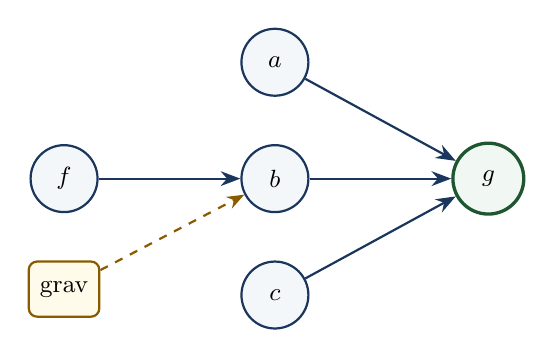
\begin{tikzpicture}[node distance=1.3cm and 1.8cm]
  \node[varnode] (f) {$f$};
  \node[paramnode, below=0.6cm of f] (grav) {$\text{grav}$};
  \node[varnode, right=of f] (b) {$b$};
  \node[varnode, above=0.6cm of b] (a) {$a$};
  \node[varnode, below=0.6cm of b] (c) {$c$};
  \node[targetnode, right=of b] (g) {$g$};
  \draw[dep] (f) -- (b);
  \draw[paramdep] (grav) -- (b);
  \draw[dep] (a) -- (g);
  \draw[dep] (b) -- (g);
  \draw[dep] (c) -- (g);
\end{tikzpicture}
\end{center}

\subsection*{Step-by-Step Derivation}

\paragraph{Steps 1--2 — Active Chain Rule.}
As in Case 1A, pruning inactive edges gives $\td{g}{f} = \pd{g}{b}\td{b}{f}$.

\paragraph{Step 3 — Dimensional Closure of Inner Node $b = \psi(f;\,\text{grav})$.}
The derivative $\td{b}{f}$ has dimension $\dimbr{b}/\dimbr{f} = (LT^{-1})/L = T^{-1}$. Searching for exponents $(\alpha_f, \alpha_{\text{grav}})$ over scope $\{f, \text{grav}\}$:
\[
  L^{\alpha_f}\,(LT^{-2})^{\alpha_{\text{grav}}} = L^0 T^{-1}
  \;\Longrightarrow\;
  \begin{cases}
    \alpha_f + \alpha_{\text{grav}} = 0,\\
    -2\alpha_{\text{grav}} = -1
  \end{cases}
  \;\Longrightarrow\;
  \alpha_{\text{grav}} = \tfrac{1}{2},\quad \alpha_f = -\tfrac{1}{2}.
\]
Hence the exact differential and integrated inner law (with $b_0 = 0$) are:
\begin{equation}
  \dd b = \kappa_b \sqrt{\frac{\text{grav}}{f}}\,\dd f
  \quad\Longrightarrow\quad
  b(f) = \int_0^f \kappa_b \sqrt{\text{grav}}\,u^{-1/2}\,\dd u = 2\kappa_b \sqrt{\text{grav}\,f}.
\end{equation}

\paragraph{Step 4 — Dimensional Closure of Outer Node $g = \Phi(a,b,c)$ with Clairaut Coupling.}
Solving $\dimbr{\beta_x} = \dimbr{g}/\dimbr{x}$ over scope $\{a, b, c\}$ yields unique monomials:
\[
  \beta_a = \kappa_{g,a}\, b^3 c, \qquad
  \beta_b = \kappa_{g,b}\, a b^2 c, \qquad
  \beta_c = \kappa_{g,c}\, a b^3.
\]
Enforcing \textbf{Clairaut exactness} across all three pairs:
\[
  \pd{\beta_a}{b} = 3\kappa_{g,a} b^2 c \stackrel{!}{=} \pd{\beta_b}{a} = \kappa_{g,b} b^2 c
  \;\implies\; \kappa_{g,b} = 3\kappa_{g,a},
  \qquad
  \pd{\beta_a}{c} = \kappa_{g,a} b^3 \stackrel{!}{=} \pd{\beta_c}{a} = \kappa_{g,c} b^3
  \;\implies\; \kappa_{g,c} = \kappa_{g,a}.
\]
Setting $\kappa_g \equiv \kappa_{g,a}$ collapses three unknown constants into \emph{one}:
\begin{equation}
  \dd g = \kappa_g\bigl(b^3 c\,\dd a + 3 a b^2 c\,\dd b + a b^3\,\dd c\bigr)
  \quad\Longrightarrow\quad
  g(a,b,c) = \kappa_g\, a b^3 c.
\end{equation}

\paragraph{Steps 5--6 — Substitution \& Integration.}
Substituting $b(f) = 2\kappa_b\sqrt{\text{grav}\,f}$ into the active rate equation $\td{g}{f} = (3\kappa_g a b^2 c)\td{b}{f}$ gives:
\begin{equation}
  \td{g}{f} = 12\,\kappa_b^3 \kappa_g\, a c\,\text{grav}^{3/2} f^{1/2}
  \quad\Longrightarrow\quad
  g(f) = 8\,\kappa_b^3 \kappa_g\, a c\, (\text{grav}\,f)^{3/2}.
\end{equation}

\begin{resultbox}{Numerical Calibration Output (\texttt{eqform})}
Dataset ($n = 60$): synthetic fluid power $g = \tfrac{1}{2} a c (2\,\text{grav}\,f)^{3/2} = \sqrt{2}\,a c (\text{grav}\,f)^{3/2}$. Fixing the inner free-fall scaling $2\kappa_b = \sqrt{2}$ ($\kappa_b = 1/\sqrt{2}$), \texttt{NumericalSolver.fit} recovers:
\begin{itemize}[leftmargin=1.4em,itemsep=2pt]
  \item \textbf{Fitted Parameter}: $\kappa_g = 0.5 \pm 1.73 \times 10^{-17}$ (exact kinetic-flux factor $\tfrac{1}{2}$!).
  \item \textbf{Goodness of Fit}: $R^2 = 1.000000$, $\text{RMSE} = 5.847 \times 10^{-12}$, $\text{BIC} = -2929.443$.
  \item \textbf{Calibrated Law}: $g = 1.41421\, a c\, f^{3/2}\,\text{grav}^{3/2} = \sqrt{2}\, a c (\text{grav}\,f)^{3/2}$.
\end{itemize}
\emph{Identifiability Note}: When $b$ is unobserved, only the product $C = 8\kappa_b^3\kappa_g$ is identifiable from $(a, c, f, g)$ data alone; measuring $b$ separately (or fixing $\kappa_b$ via kinematics) separates $\kappa_b$ from $\kappa_g$.
\end{resultbox}

% ============================================================================
\section{Case 2: Linear \& Non-Linear Kinematics (\texttt{ch1.tex}, Sec.~1)}
% ============================================================================

\begin{setupbox}{Problem Statement — Reproducing \texttt{ch1.tex} Eq.~(2.1)--(2.6)}
\textbf{Given}: Displacement $s = f(v)$ ($L$), velocity $v = g(t)$ ($LT^{-1}$), time $t$ ($T$), constant acceleration $a$ ($LT^{-2}$), and kinematic rate identities $\td{s}{t} \equiv v$ and $\td{v}{t} \equiv a$.\\
\textbf{Goal}: Recover the equations of uniformly accelerated motion $v(t)$ and $s(t)$ without knowing them in advance.
\end{setupbox}

\subsection*{Step-by-Step Derivation}

\paragraph{Step 1 — Chain Rule.}
Expanding $s(v(t))$ with respect to $t$:
\begin{equation}
  \td{s}{t} = \pd{s}{v}\td{v}{t}.
\end{equation}

\paragraph{Step 2 — Rate-Identity Dimensional Closure for $v(t)$.}
Substituting the known definitions $\td{s}{t} = v$ and $\td{v}{t} = a$, the chain rule becomes an affine regression model $v = v_0 + \beta_1 a$. Matching dimensions on the slope $\beta_1$:
\[
  \dimbr{\beta_1} = \frac{\dimbr{v}}{\dimbr{a}} = \frac{LT^{-1}}{LT^{-2}} = T \;\Longrightarrow\; \beta_1 = \kappa_v t.
\]
Setting unit scaling $\kappa_v = 1$ (since $a$ is defined as $\td{v}{t}$) yields \texttt{ch1.tex} Eq.~(2.5):
\begin{equation}
  v(t) = v_0 + a t.
\end{equation}

\paragraph{Step 3 — Integration to Displacement $s(t)$.}
Integrating $\td{s}{t} = v(t) = v_0 + a t$ with respect to $t$ introduces the initial displacement $s_0$ and yields \texttt{ch1.tex} Eq.~(2.6):
\begin{equation}
  s(t) = s_0 + \int_0^t (v_0 + a\tau)\,\dd\tau = s_0 + v_0 t + \frac{1}{2} a t^2.
\end{equation}

\begin{insightbox}{Class Note — Cleaning Up \texttt{ch1.tex} Eq.~(2.6)}
In the original draft of \texttt{ch1.tex} (line~69), the intermediate integral was written loosely as $s = \beta_1 \int_0^t \dd v$. Because $\beta_1 = t$ is itself a function of the integration variable, it cannot be pulled outside the integral. Integrating $\td{s}{t} = v(t)$ directly with respect to $t$ produces the exact factor $\tfrac{1}{2}at^2$ rigorously and automatically preserves the initial position $s_0$.
\end{insightbox}

% ============================================================================
\section{Case 3: Variable-Mass Momentum (\texttt{ch1.tex}, Sec.~2)}
% ============================================================================

\begin{setupbox}{Problem Statement — Reproducing \texttt{ch1.tex} Eq.~(2.7)--(2.11)}
\textbf{Given}: Momentum $p = f(m, v)$ with $\dimbr{p} = MLT^{-1}$, mass $m$ ($M$), and velocity $v$ ($LT^{-1}$).\\
\textbf{Goal}: Derive both the total differential $\dd p$ (governing variable-mass rockets/glaciers) and the state law $p(m, v)$.
\end{setupbox}

\subsection*{Step-by-Step Derivation}

\paragraph{Step 1 — Exact Differential.}
Without assuming $m$ or $v$ is constant:
\begin{equation}
  \dd p = \pd{p}{m}\,\dd m + \pd{p}{v}\,\dd v.
\end{equation}

\paragraph{Step 2 — Dimensional Closure \& Clairaut Coupling.}
Over scope $\{m, v\}$:
\[
  \dimbr{\pd{p}{m}} = \frac{MLT^{-1}}{M} = LT^{-1} \implies \beta_m = \kappa_{p,m}\,v,
  \qquad
  \dimbr{\pd{p}{v}} = \frac{MLT^{-1}}{LT^{-1}} = M \implies \beta_v = \kappa_{p,v}\,m.
\]
Applying Clairaut symmetry $\pd{\beta_m}{v} = \pd{\beta_v}{m}$ gives $\kappa_{p,m} = \kappa_{p,v} \equiv \kappa_p$. With unit definition $\kappa_p = 1$:
\begin{equation}
  \dd p = v\,\dd m + m\,\dd v.
\end{equation}

\paragraph{Step 3 — Integration \& Rate Form.}
Integrating the exact differential (with $p_0 = 0$) recovers $p = mv$. Dividing the differential by $\dd t$ immediately yields Newton's variable-mass second law (\texttt{ch1.tex} Eq.~2.10):
\begin{equation}
  F \equiv \td{p}{t} = v\td{m}{t} + m\td{v}{t}.
\end{equation}

% ============================================================================
\section{Case 4: Kinetic Energy \& Numerical Discovery of $\tfrac{1}{2}$ (\texttt{ch1.tex}, Sec.~3.1)}
% ============================================================================

\begin{setupbox}{Problem Statement — From Dimensional Scaling to Exact Prefactor}
\textbf{Given}: Kinetic energy $K = f(m, v)$ with $\dimbr{K} = ML^2T^{-2}$, mass $m$ ($M$), velocity $v$ ($LT^{-1}$).\\
\textbf{Goal}: Show what pure dimensional analysis + Clairaut exactness can determine symbolically, and what requires numerical data.
\end{setupbox}

\subsection*{Step-by-Step Derivation}

\paragraph{Step 1 — Dimensional Closure.}
Over scope $\{m, v\}$, the partial derivative slots have unique dimensions:
\[
  \dimbr{\pd{K}{m}} = \frac{ML^2T^{-2}}{M} = L^2T^{-2} \implies \beta_m = \kappa_{K,m}\,v^2,
  \qquad
  \dimbr{\pd{K}{v}} = \frac{ML^2T^{-2}}{LT^{-1}} = MLT^{-1} \implies \beta_v = \kappa_{K,v}\,mv.
\]

\paragraph{Step 2 — Clairaut Exactness Locks the 2:1 Ratio!}
Before touching any data, enforce mixed-partial symmetry:
\[
  \pd{\beta_m}{v} = 2\kappa_{K,m}\,v \;\stackrel{!}{=}\; \pd{\beta_v}{m} = \kappa_{K,v}\,v
  \quad\Longrightarrow\quad
  \kappa_{K,v} = 2\kappa_{K,m}.
\]
Thus, writing $\kappa_K \equiv \kappa_{K,m}$, the exact differential and integrated potential are:
\begin{equation}
  \dd K = \kappa_K\, v^2\,\dd m + 2\kappa_K\, m v\,\dd v
  \quad\Longrightarrow\quad
  K(m, v) = \kappa_K\, m v^2.
\end{equation}

\begin{resultbox}{Numerical Discovery of the $\tfrac{1}{2}$ Factor (\texttt{eqform})}
Dimensional analysis alone can never fix a dimensionless constant like $\tfrac{1}{2}$. Feeding $n = 40$ observations of $(m, v, K)$ into \texttt{NumericalSolver.fit} solves exact Ordinary Least Squares in one step:
\begin{itemize}[leftmargin=1.4em,itemsep=2pt]
  \item \textbf{Fitted Parameter}: $\kappa_K = 0.5 \pm 3.58 \times 10^{-17}$.
  \item \textbf{Goodness of Fit}: $R^2 = 1.000000$, $\text{RMSE} = 2.956 \times 10^{-12}$, $\text{BIC} = -2006.570$.
  \item \textbf{Calibrated Law}: $\displaystyle K = \frac{1}{2} m v^2$.
\end{itemize}
\end{resultbox}

% ============================================================================
\section{Case 5: Blasius Boundary Layer \& Buckingham-$\Pi$ Discovery (\texttt{ch1.tex}, Eq.~2.23)}
% ============================================================================

\begin{setupbox}{Problem Statement — Underdetermined Systems ($\text{nullity} > 0$)}
\textbf{Given}: Boundary-layer thickness $\delta$ ($L$) over a flat plate depends on downstream position $x$ ($L$), governed by fluid density $\rho$ ($ML^{-3}$), free-stream velocity $v$ ($LT^{-1}$), and dynamic viscosity $\mu$ ($ML^{-1}T^{-1}$).\\
\textbf{Goal}: Discover the dimensionless Reynolds number $Re$ automatically and identify the exact Blasius law $\delta = 5.0\,x/\sqrt{Re}$ from data.
\end{setupbox}

\subsection*{Step-by-Step Derivation}

\paragraph{Steps 1--4 — Leading Monomial \& Nullspace Analysis.}
There are $m = 4$ scope variables $\{x, \rho, v, \mu\}$ across $k = 3$ base dimensions $\{M, L, T\}$. The dimension matrix is:
\[
  D = \bordermatrix{
    & x & \rho & v & \mu \cr
    M & 0 & 1 & 0 & 1 \cr
    L & 1 & -3 & 1 & -1 \cr
    T & 0 & 0 & -1 & -1
  },
  \qquad \text{rank}(D) = 3, \quad \text{nullity}(D) = 4 - 3 = 1.
\]
For $\dimbr{\pd{\delta}{x}} = L/L = 1$ (dimensionless), the minimum-complexity particular solution is $\boldsymbol{\alpha}^{(p)} = [0, 0, 0, 0]^T$, giving leading law $\delta = \kappa_\delta x$.

\paragraph{Step 5 — Automatic Reynolds Number Extraction.}
Because $\text{nullity}(D) = 1$, \texttt{DimensionalEngine} computes the canonical coprime integer nullspace vector $\mathbf{n}_1 = [1, 1, 1, -1]^T$, automatically discovering the \textbf{Reynolds number}:
\begin{equation}
  \Pi_1 = \frac{\rho v x}{\mu} \equiv Re.
\end{equation}
\texttt{SymbolicSolver} therefore emits three competing candidate laws:
\begin{enumerate}[leftmargin=1.5em,itemsep=2pt]
  \item \texttt{leading\_dimensional}: $\delta = \kappa_\delta x$ \quad (ignores viscous effects).
  \item \texttt{buckingham\_pi\_power}: $\delta = \kappa_\delta x \left(\frac{\rho v x}{\mu}\right)^{\nu_1}$ \quad (power-law $\Pi$-modulation).
  \item \texttt{buckingham\_pi\_affine}: $\delta = \kappa_\delta x \left(1 + \lambda_1 \frac{\rho v x}{\mu}\right)$ \quad (first-order linear $\Pi$-series).
\end{enumerate}

\subsection*{Numerical Model Selection by BIC}
Evaluating all three candidates against $n = 80$ laminar-plate observations ($\delta = 5.0\,x/\sqrt{Re}$), \texttt{NumericalSolver.rank\_candidates} fits each candidate (using analytic-Jacobian Trust-Region NLLS for the nonlinear exponent $\nu_1$) and ranks them by BIC:

\begin{center}
\renewcommand{\arraystretch}{1.25}
\begin{tabular}{@{}clrrrl@{}}
\toprule
\textbf{Rank} & \textbf{Candidate} & \textbf{$R^2$} & \textbf{RMSE} & \textbf{BIC} & \textbf{Calibrated Parameters} \\
\midrule
\textbf{\#1} & \texttt{buckingham\_pi\_power} & \textbf{1.000000} & \textbf{$8.25\times 10^{-15}$} & \textbf{$-4952.815$} & $\kappa_\delta = 5.0,\;\; \nu_1 = -0.5$ \\
\#2 & \texttt{buckingham\_pi\_affine} & $0.725787$ & $1.37\times 10^{-3}$ & $-819.544$ & $\kappa_\delta = 0.0101,\;\; \lambda_1 = -4.75\times 10^{-7}$ \\
\#3 & \texttt{leading\_dimensional} & $0.054758$ & $2.54\times 10^{-3}$ & $-724.923$ & $\kappa_\delta = 0.00641$ \\
\bottomrule
\end{tabular}
\end{center}

\begin{resultbox}{Discovered Blasius Equation (\texttt{ch1.tex} Eq.~2.23)}
The winning candidate (\textbf{\#1}, lower BIC by $>4100$ points) recovers the exact Blasius laminar boundary-layer thickness law without prior fluid-mechanics equations:
\[
  \delta = 5\,\sqrt{\frac{\mu x}{\rho v}} = \frac{5.0\,x}{\sqrt{Re}}.
\]
\end{resultbox}

% ============================================================================
\section{Case 6: Beyond Physics — SaaS Economics with Custom Dimensions}
% ============================================================================

\begin{setupbox}{Problem Statement — Domain-Agnostic Formulation}
\textbf{Given}: Monthly recurring revenue $R$ (\texttt{USD/Month}) depends on active users $U$ (\texttt{Users}) and average revenue per user $P$ (\texttt{USD/(Users*Month)}). Active users $U$ depend on marketing spend $S$ (\texttt{USD}) governed by customer acquisition cost $\text{CAC}$ (\texttt{USD/Users}).\\
\textbf{Goal}: Express monthly revenue $R$ as a function of marketing spend $S$.
\end{setupbox}

\begin{center}
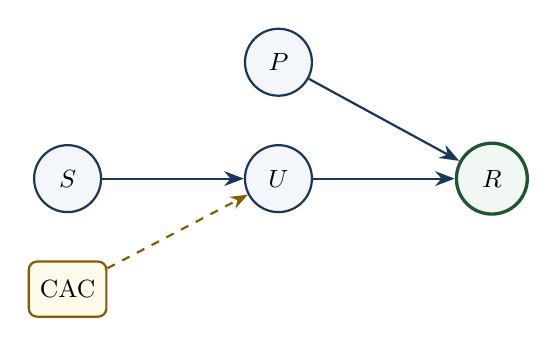
\begin{tikzpicture}[node distance=1.3cm and 1.8cm]
  \node[varnode] (S) {$S$};
  \node[paramnode, below=0.6cm of S] (CAC) {$\text{CAC}$};
  \node[varnode, right=of S] (U) {$U$};
  \node[varnode, above=0.6cm of U] (P) {$P$};
  \node[targetnode, right=of U] (R) {$R$};
  \draw[dep] (S) -- (U);
  \draw[paramdep] (CAC) -- (U);
  \draw[dep] (U) -- (R);
  \draw[dep] (P) -- (R);
\end{tikzpicture}
\end{center}

\subsection*{Step-by-Step Derivation}

\paragraph{Steps 1--2 — Active Chain Rule.}
With price $P$ independent of marketing spend $S$, active path pruning along $S \to U \to R$ yields:
\begin{equation}
  \td{R}{S} = \pd{R}{U}\,\td{U}{S}.
\end{equation}

\paragraph{Steps 3--4 — Custom-Unit Dimensional Closure.}
Using the custom base dimensions $\{\texttt{USD},\, \texttt{Users},\, \texttt{Month}\}$:
\begin{align}
  \dimbr{\td{U}{S}} &= \frac{\texttt{Users}}{\texttt{USD}} = \dimbr{\text{CAC}}^{-1}
  \;\Longrightarrow\; \dd U = \frac{\kappa_U}{\text{CAC}}\,\dd S
  \;\Longrightarrow\; U(S) = U_0 + \kappa_U \frac{S}{\text{CAC}},\\[4pt]
  \dimbr{\pd{R}{U}} &= \frac{\texttt{USD/Month}}{\texttt{Users}} = \dimbr{P},\qquad
  \dimbr{\pd{R}{P}} = \dimbr{U}.
\end{align}
Clairaut exactness on $R(U, P)$ couples both partials to a single efficiency constant $\kappa_R$:
\begin{equation}
  \dd R = \kappa_R\bigl(P\,\dd U + U\,\dd P\bigr)
  \;\Longrightarrow\;
  R(U, P) = R_0 + \kappa_R\, U P.
\end{equation}

\paragraph{Steps 5--6 — Marginal Return \& Integrated Revenue Function.}
Composing $U(S)$ into $R(U, P)$ yields both the marginal revenue per marketing dollar and the full revenue equation:
\begin{equation}
  \td{R}{S} = \frac{\kappa_R \kappa_U P}{\text{CAC}},
  \qquad
  R(S) = R_0 + \kappa_R P \left(U_0 + \kappa_U \frac{S}{\text{CAC}}\right).
\end{equation}

\begin{insightbox}{Economic Interpretation of Every Term}
\begin{itemize}[leftmargin=1.4em,itemsep=2pt]
  \item $R_0$: Non-user baseline revenue (e.g., platform/enterprise licensing fees).
  \item $\kappa_R P U_0$: Recurring revenue from existing organic/initial users $U_0$.
  \item $\frac{\kappa_R \kappa_U P}{\text{CAC}}\,S$: Incremental monthly revenue from paid acquisition, where $\frac{P}{\text{CAC}}$ is the inverse payback period in months$^{-1}$ and $\kappa_R, \kappa_U$ capture retention/conversion efficiency!
\end{itemize}
\end{insightbox}

% ============================================================================
\section{Summary Reference \& Student Practice Problems}
% ============================================================================

\begin{center}
\renewcommand{\arraystretch}{1.25}
\footnotesize
\begin{tabularx}{\textwidth}{@{}l l l X@{}}
\toprule
\textbf{Case} & \textbf{Dependency Graph} & \textbf{Key Mechanism} & \textbf{Formulated / Calibrated Law} \\
\midrule
1A & $g(a,b,c),\; b(f)$ & Dimension-free closures & Affine Taylor \& Power-Law scaling in $(a,c,f)$ \\
1B & $g(a,b,c),\; b(f;\,\text{grav})$ & Clairaut + OLS fit & $g = \sqrt{2}\,a c (\text{grav}\,f)^{3/2}$ \\
2 & $s(v),\; v(t)$ & Rate identities + integration & $v = v_0 + at,\quad s = s_0 + v_0 t + \tfrac{1}{2}at^2$ \\
3 & $p(m,v)$ & Clairaut exactness & $\dd p = v\,\dd m + m\,\dd v \implies p = mv$ \\
4 & $K(m,v)$ & Clairaut 2:1 + OLS fit & $K = \kappa_K mv^2 \xrightarrow{\text{fit}} \tfrac{1}{2}mv^2$ \\
5 & $\delta(x;\,\rho,v,\mu)$ & Buckingham-$\Pi$ + BIC & $\Pi_1 = Re,\quad \delta = 5.0\,x/\sqrt{Re}$ \\
6 & $R(U,P),\; U(S;\,\text{CAC})$ & Custom domain units & $R = R_0 + \kappa_R P\bigl(U_0 + \kappa_U S/\text{CAC}\bigr)$ \\
\bottomrule
\end{tabularx}
\end{center}

\subsection*{Recommended Exercises Using \texttt{eqform}}
\begin{enumerate}[leftmargin=1.5em,itemsep=4pt]
  \item \textbf{Pendulum Period}: Formulate $T = \Phi(\ell;\, \text{grav}, m)$ with $\dimbr{T}=T$, $\dimbr{\ell}=L$, $\dimbr{\text{grav}}=LT^{-2}$, $\dimbr{m}=M$. Verify that $m$ automatically receives exponent $0$ and calibrate $\kappa_T = 2\pi$ from synthetic data.
  \item \textbf{Hydroelectric Power (\texttt{ch1.tex} Sec.~3.3)}: Express $P = \Phi(\rho, Q, h;\, \text{grav})$ and verify that \texttt{eqform} yields $P = \eta \rho g Q h$ with $E_{P,Q} = E_{P,h} = 1$ via \texttt{NumericalSolver.elasticities}.
  \item \textbf{Multi-Path Diamond Graph}: Declare $p = \Phi(m, v)$, $m = \psi_1(t;\,\dot{m})$, $v = \psi_2(t;\,a)$ and inspect how both paths $t \to m \to p$ and $t \to v \to p$ sum in $\td{p}{t}$.
\end{enumerate}

\end{document}
